% 导数与函数极值
% 微积分|导数|极值|鞍点|驻点

\pentry{二阶导数\upref{HigDer}}
\begin{figure}[ht]
\vskip-10pt
\centering
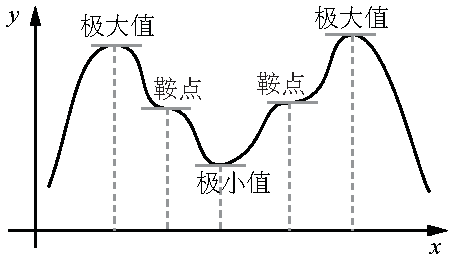
\includegraphics[width=7.5cm]{./figures/DerMax_1.pdf}
\caption{导数为零的三种点}\label{DerMax_fig1}
\end{figure}

如\autoref{DerMax_fig1}, 若一个一元函数 $y = f(x)$ 在某区间内处处可导(即对区间内的任何 $x$ 导数 $f'(x)$ 都存在),若区间内存在某些 $x_i$ 能使 $f'(x_i) = 0$( 即在这些点处函数曲线的斜率为零), 这样的点被称为\textbf{驻点}.

而从函数曲线来看,驻点又分为三类: \textbf{极大值},\textbf{极小值},\textbf{鞍点}. 我们以 $x_i$ 为中心取一个小区间, 如果这个区间足够小, 那么容易看出对于极大值点, $f'(x)$ 在小区间内递减, 对于鞍点, $f'(x)$ 在小区间内恒为非负或恒为非正, 对于极小值点, $f'(x)$ 在小区间内递增. 所以为了判断驻点的类型, 我们可以在驻点处求函数的二阶导数 $f''(x_i)$. 假设二阶偏导存在, 如果 $f''(x_i) < 0$, 那么 $x_i$ 是极大值点, 如果 $f''(x_i) > 0$, $x_i$ 是极小值点. 要注意的是, 如果 $f''(x_i) = 0$, 不能直接判断 $x_i$  鞍点, 需要进一步分析: 例如我们可以判断驻点左边和右边的一阶导数符号, 如果同号则是驻点, 左正右负则是极大值, 左负右正则是极小值.

另外, 若某个极小值点是整个考察区间中函数值最小的点, 它就被称为\textbf{最小值点}, 若某个极大值点是该区间中函数值最大的点, 它就被称为\textbf{最大值点}.

\begin{example}{}
二次函数 $f(x) = ax^2 + bx + c$ 的导函数为 $f'(x) = 2ax + b$, 所以唯一的驻点为 $-b/(2a)$. 函数的二阶导数是一个常数 $f''(x) = 2a$, 所以当 $a > 0$ 时驻点是唯一的极小值点, 即最小值点. 同理, 当 $a < 0$ 时驻点是最大值点.
\end{example}

\begin{figure}[ht]
\centering
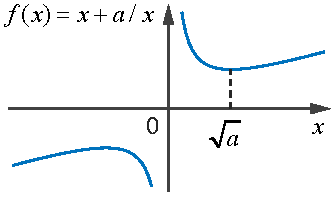
\includegraphics[width=6cm]{./figures/DerMax_2.pdf}
\caption{\autoref{DerMax_ex2} 函数图} \label{DerMax_fig2}
\end{figure}

\begin{example}{}\label{DerMax_ex2}
函数 $f(x) = x+a/x \ \ (a > 0)$ 的一阶导函数为 $f'(x) = 1 - a/x^2$, 若我们只考察区间 $(0, +\infty)$, 唯一的驻点为 $x = \sqrt{a}$. 函数的二阶导函数 $f''(x) = 2a/x^3$ 在驻点处的值为 $2/\sqrt{a} > 0$, 所以该驻点为当前区间的最小值点(\autoref{DerMax_fig2}).
\end{example}

\begin{example}{}\label{DerMax_ex3}
函数 $f(x) = x^3$ 的一阶导函数为 $f'(x) = 3x^2$, 唯一的驻点为 $x = 0$. 函数的二阶导函数 $f''(x) = 6x$ 在驻点处的值为 $0$. 由于 $f'(x)$ 在原点左侧和右侧都大于 0, 所以这是一个鞍点.
\end{example}
